\section{Geometria vettoriale}

\subsection{Introduzione}
%%%%%%%%%%%%%%%%%%%%%%%%%%%%%%%%%%%%%%%%%%%%%%%%%%%%%%%%%%%%%%%%%%%%%%
%\subfile{../ch/BS-MPT-FP-rappel-fct-1-2}
\begin{questions}

	\begin{qblock}
		\question
		\exonly{Determinare dove costruire un ponte $HG$ perpendicolare al fiume così da minimizzare la distanza tra $A$ e $B$.
		}
		\begin{tikzpicture}[baseline={($(current bounding box.north)-(0,1.6ex)$)}, scale=1.5]

			\draw[-] (-4,0)-- (3.5,0);
			\draw[-,name path=river] (-4,1)-- (3.5,1);
			\fill (-3,2) coordinate[label=above:$A$] (A)  circle (1pt);
			\fill (-2,1) coordinate[label=above:$H$] (H) circle (1pt);
			\fill (-2,0) coordinate[label=above:$G$] (G) circle (1pt);
			\fill (2,-2) coordinate[label=above:$B$] (B)  circle (1pt);
			\draw[dotted] (A) -- (H) --(G) --(B);
			\ifprintanswers
				\coordinate (B1) at ($(B)+(0,1)$);
				\path[name path=shortpath] (B1) -- (A);
				\path [name intersections={of=shortpath and river,by=G1}];
				\draw[red] (A) -- (G1) -- ++(0,-1) -- (B) ;
				\draw[red,dashed] (B) -- (B1) -- (A);

			\fi
		\end{tikzpicture}

		\solonly{Discussione in classe }
	\end{qblock}

	\begin{qblock}
		\question
		\exonly{Consideriamo i vettori rappresentati: }
		%\solonly{\hfill}
		\begin{parts}
			\part
			\exonly{
				Quali vettori sono uguali? }

			\solonly{
				$\vec{a}$ e $\vec{d}$
			}

			\part
			\exonly{
				Quali vettori hanno la stessa intensità?
			}

			\solonly{
				$\vec{a}$ , $\vec{d}$ e $\vec{e}$

				$\vec{b}$ e $\vec{c}$
			}

			\part
			\exonly{
				Quali vettori sono opposti?
			}
			\solonly{
				$\vec{b}$ e $\vec{c}$
			}

			\begin{tikzpicture}[baseline={($(current bounding box.north)-(0,1.6ex)$)}]
				\ifprintanswers   \else
					\begin{axis}[
							AxisDefaults,
							TinyAxisLabels,
							xmin=-6,
							xmax=6,
							ymin=-6,
							ymax=6,
							yticklabels={},
							xticklabels={},
						]
						\addplot[black] {0};
						\draw[->] (axis cs:-2,3)-- node[midway,above]{$\vec{a}$} +(axis direction cs:2,1);
						\draw[->] (axis cs:-5,-4)--node[midway,above]{$\vec{b}$}  +(axis direction cs:1,4);
						\draw[->] (axis cs:3,-1)--node[midway,above]{$\vec{c}$} +(axis direction cs:-1,-4);
						\draw[->] (axis cs:3,-5)-- node[midway,above]{$\vec{d}$}  +(axis direction cs:2,1);
						\draw[->] (axis cs:1,1)-- node[midway,above]{$\vec{e}$} +(axis direction cs:2,-1);
					\end{axis}
				\fi
			\end{tikzpicture}

		\end{parts}
	\end{qblock}

	\begin{qblock}
		\question
		\exonly{
			Consideriamo le forze $\vec{F_1}$ e $\vec{F_2}$. Determinare graficamente e algebricamente il vettore della forza $\vec{F_3}$ tale per cui $\vec{F_1}+\vec{F_2}+\vec{F_3}=\vec{0}$.}



		\begin{tikzpicture}[baseline={($(current bounding box.north)-(0,1.6ex)$)}]

			\draw[->] (0,0)-- node[midway,above]{$\vec{F_1}$} +(3,2);
			\draw[->] (0,0)--node[midway,above]{$\vec{F_2}$}  +(-2,1);
			\ifprintanswers
				\draw[->,red] (0,0)--node[midway,above]{$\vec{F_3}$}  +(-1,-3);
			\fi
		\end{tikzpicture}

		\solonly{$\vec{F_3}=-\left( \vec{F_1}+\vec{F_2} \right) $}
	\end{qblock}

	\begin{qblock}
		\question
		\exonly{
			Consideriamo le forze $\vec{F_1}$ e $\vec{F_2}$. Determinare graficamente e algebricamente il vettore della forza $\vec{F_3}$ tale per cui $\vec{F_1}+\vec{F_2}+\vec{F_3}=\vec{R}$.}


		\begin{tikzpicture}[baseline={($(current bounding box.north)-(0,1.6ex)$)}]

			\draw[->] (0,0)-- node[midway,above]{$\vec{F_1}$} +(3,2);
			\draw[->] (0,0)--node[midway,above]{$\vec{F_2}$}  +(-2,1);
			\draw[->] (0,0)--node[midway,above]{$\vec{R}$}  +(-2,4);
			\ifprintanswers
				\draw[->,blue] (3,2)--node[midway,above]{$\vec{F_2}$}  +(-2,1);
				\draw[->,red] (1,3)--node[midway,above]{$\vec{F_3}$}  +(-3,1);
			\fi
		\end{tikzpicture}

		\solonly{$\vec{F_3}=\vec{R}-\left( \vec{F_1}+\vec{F_2} \right) $}
	\end{qblock}

\end{questions}

\exnewpage
\subsection{Componenti, operazioni di base}

\begin{questions}


	\begin{qblock}
		\question
		\exonly{Determinare le componenti dei vettori $\vec{a}$, $\vec{b}$ e $\vec{c}$

			\begin{tikzpicture}[baseline={($(current bounding box.north)-(0,1.6ex)$)}]

				\begin{axis}[
						AxisDefaults,
						TinyAxisLabels,
						width=\linewidth,
						xmin=-8,
						xmax=8,
						ymin=-8,
						ymax=8,
						yticklabels={},
						xticklabels={},
					]
					\addplot[black] {0};
					\draw[->] (axis cs:-6,1)-- node[midway,above]{$\vec{a}$} +(axis direction cs:8,5);
					\draw[->] (axis cs:7,-7)--node[midway,left]{$\vec{b}$}  +(axis direction cs:0,9);
					\draw[->] (axis cs:3,1)--node[midway,left]{$\vec{c}$} +(axis direction cs:-2,-8);
					\draw[->,thick] (axis cs:3,3)-- node[midway,above]{$\vec{u}$}  +(axis direction cs:2,-1);
					\draw[->,thick] (axis cs:3,3)-- node[midway,left]{$\vec{v}$} +(axis direction cs:1,4);
				\end{axis}
			\end{tikzpicture}
		}
		%\solonly{\hfill}

		\begin{parts}
			\part
			\exonly{rispetto alla base $\left(\vec{u},\vec{v} \right)$}
			\solonly{
				$\vec{a}=\vecII{3}{2}$, $\vec{a}=\vecII{-1}{2}$, $\vec{c}=\vecII{0}{-2}$
			}
			\part
			\exonly{rispetto alla standard}
			\solonly{
				$\vec{a}=\vecII{8}{5}$, $\vec{a}=\vecII{0}{9}$, $\vec{c}=\vecII{-2}{-8}$
			}
		\end{parts}
	\end{qblock}


	\begin{qblock}
		\question
		\exonly{Dati i vettori $\vec{a}=\vecII{3}{5}$, $\vec{b}=\vecII{-4}{2}$ e $\vec{c}=\vecII{-3}{-4}$ determinare le componenti di

			$\vec{d}=\vec{a}+\vec{b}+\vec{c}$, $\vec{e}=\vec{a}-\vec{b}-\vec{c}$, $\vec{f}=\frac{1}{2}\vec{a}$ e $\vec{g}=-\dfrac{3}{2}\vec{c}$

		}

		\solonly{$\vec{d}=\vecII{-4}{3}$, $\vec{e}=\vecII{10}{7}$, $\vec{f}=\vecII{\sfrac{3}{2}}{\sfrac{5}{2}}$ e $\vec{g}=\vecII{\sfrac{9}{2}}{6}$}

		\question
		\exonly{Dati i vettori $\vec{a}=\vecII{2}{3}$, $\vec{b}=\vecII{-4}{2}$.

			Calcolare $\norm{\vec{a}}$, $\norm{\vec{b}}$, $\norm{\vec{a}+\vec{b}}$ e $\norm{\vec{a}}+\norm{\vec{b}}$}
		\solonly{$\norm{\vec{a}}=\sqrt{13}$, $\norm{\vec{b}}=\sqrt{20}$, $\norm{\vec{a}+\vec{b}}=\sqrt{29}\approx \num{5.39}$ e $\norm{\vec{a}}+\norm{\vec{b}}\approx \num{8.07}$}
	\end{qblock}


	\begin{qblock}
		\question
		\exonly{
			Dati i vettori $\vec{v}=\vecII{3}{-5}$e $\vec{w}=\vecII{-2}{3}$ calcolare:
		}
		%\solonly{\hfill}
		\begin{multicols}{2}
			\begin{parts}
				\part
				\exonly{$\vec{v}+\vec{w}$}
				\solonly{$\vecII{1}{-2}$}

				\part
				\exonly{$\vec{w}-\vec{v}$}
				\solonly{$\vecII{-5}{8}$}

				\part
				\exonly{$-5\vec{v}$}
				\solonly{$\vecII{-15}{25}$}

				\part
				\exonly{$\norm{\vec{v}}$}
				\solonly{$\sqrt{34}$}

				\part
				\exonly{$2\vec{v}+3\vec{w}$}
				\solonly{$\vecII{0}{-1}$}

				\part
				\exonly{$3\vec{v}-2\vec{w}$}
				\solonly{$\vecII{13}{-21}$}

				\part
				\exonly{$\norm{\vec{v}-\vec{w}}$}
				\solonly{$\sqrt{89}$}

				\part
				\exonly{$\norm{\vec{v}}-\norm{\vec{w}}$}
				\solonly{$\sqrt{34}-\sqrt{13}$}


				\part
				\exonly{$\norm{5\vec{v}}$}
				\solonly{$5\sqrt{34}$}

				\part
				\exonly{$\norm{-5\vec{v}}$}
				\solonly{$5\sqrt{34}$}
			\end{parts}
		\end{multicols}
	\end{qblock}


	\begin{qblock}
		\question
		\exonly{Sono dati due vettori  $\vec{a}$ e $\vec{b}$ (vedi schizzo sotto) con $\norm{\vec{a}}=2$ e $\norm{\vec{b}}=3$.

			\begin{tikzpicture}[baseline={($(current bounding box.north)-(0,1.6ex)$)}]
				\draw[-latex] (-3,0) -- (3,0) coordinate (X);
				\draw[-latex] (0,-3) -- (0,3);
				\draw[->] (0,0) coordinate (O)-- node[midway,above]{$\vec{a}$} +(1,2) coordinate (A);
				\draw[->] (O)--node[midway,above]{$\vec{b}$}  +(-3,-2) coordinate (B);
				\draw pic["$70\degree$",draw, angle eccentricity=1.5, blue] {angle=X--O--A};
				\draw pic["$150\degree$",draw, angle radius=0.7cm,angle eccentricity=1.5, blue] {angle=B--O--X};
			\end{tikzpicture}
		}

		\begin{parts}
			\part

			\exonly{Calcolare le componenti in base standard dei vettori $\vec{a}$ e $\vec{b}$. Approssimare il risultati a due decimali. }
			\solonly{$\vec{a} \approx \vecII{\num{0.68}}{\num{1.88}}$, $\vec{b} \approx \vecII{\num{-2.6}}{\num{-1.5}}$}

			\part
			\exonly{ Determinare il vettore posizione $\overrightarrow{OC} =\vec{a}+\vec{b}$.  }

			\solonly{ $\overrightarrow{OC}=\vecII{\num{-1.92}}{\num{0.38}}$  }

			\part
			\exonly{Esprimere le coordinate di $C$ in forma polare. }
			\solonly{$C$: $1.96 \angle \ang{168.8}$}

		\end{parts}
	\end{qblock}


	\begin{qblock}
		\question
		\exonly{
			Ad un certo instante un aeroplano vola ad una velocità di
			\SI{700}{\kilo\meter/\hour} e il pilota punta in direzione nord. Ad un tratto un vento di \SI{120}{\kilo\meter/\hour}
			proveniente da est ne perturba la traiettoria.
			Calcolare l'intensità e la direzione della velocità dell'aeroplano nel momento cui incontra la perturbazione.
		}
		\solonly{Velocità al suolo di \SI{710.21}{\kilo\meter/\hour} in direzione $\num{9.7}\degree  NO$}

		\question
		\exonly{Dato i punti $A(2;3)$, $B(-1;2)$ e $C(5;-4)$ determinare le componenti dei vettori $\overrightarrow{AB}$,$\overrightarrow{BC}$ e $\overrightarrow{AC}$}
		\solonly{$\overrightarrow{AB}=\vecII{-3}{-1}$,$\overrightarrow{BC}=\vecII{6}{-6}$ e $\overrightarrow{AC}=\vecII{3}{-7}$}
	\end{qblock}


	\begin{qblock}
		\question
		\exonly{Date le coordinate $A(1;-1)$, $B(2;2)$, $C(-3;2)$ , $D(-4;-1)$ e $E(0,2)$. }

		\begin{parts}
			\part
			\exonly{Determinare la natura del quadrilatero $ABCD$ (quadrilatero qualunque, trapezio, parallelogrammo, rettangolo, quadrato)}
			\solonly{

				\begin{tikzpicture}[baseline={($(current bounding box.north)-(0,1.6ex)$)},scale=0.5]
					\draw[] (-3,2) coordinate[label=left:$C$] (C) -- (2,2) coordinate[label=right:$B$] (B) -- (1,-1) coordinate[label=right:$A$] (A) -- (-4,-1) coordinate[label=left:$D$] (D) -- cycle;
				\end{tikzpicture}

				Parallelogrammo: $ \overrightarrow{AB} = \overrightarrow{DC}$}
			\part
			\exonly{Determinare la natura del quadrilatero $ABED$ (quadrilatero qualunque, trapezio, parallelogrammo, rettangolo, quadrato)}
			\solonly{

				\begin{tikzpicture}[baseline={($(current bounding box.north)-(0,1.6ex)$)},scale=0.5]
					\draw[] (0,2) coordinate[label=left:$E$] (E) -- (2,2) coordinate[label=right:$B$] (B) -- (1,-1) coordinate[label=right:$A$] (A) -- (-4,-1) coordinate[label=left:$D$] (D) -- cycle;
				\end{tikzpicture}

				Trapezio: $ \overrightarrow{AD} =\frac{5}{2} \overrightarrow{BE}$

			}
		\end{parts}
	\end{qblock}


	\begin{qblock}
		\question
		\exonly{Dati $A(2;3;-1)$, $B(-1;5;2)$ e $C(-3;4;1)$}

		\begin{parts}
			\part
			\exonly{Determinare le componenti di $\overrightarrow{AB}$, $\overrightarrow{AC}$ e $\overrightarrow{BC}$}
			\solonly{$\overrightarrow{AB}=\vecIII{-3}{2}{3}$, $\overrightarrow{AC}=\vecIII{-5}{1}{2}$ e $\overrightarrow{BC}=\vecIII{-2}{-1}{-1}$}

			\part
			\exonly{Calcolare la norma di $\overrightarrow{AB}$, $\overrightarrow{AC}$ e $\overrightarrow{BC}$}
			\solonly{$\norm{\overrightarrow{AB}}=\sqrt{22}$, $\norm{\overrightarrow{AC}}=\sqrt{30}$ e $\norm{\overrightarrow{BC}}=\sqrt{6}$}

		\end{parts}
	\end{qblock}

\end{questions}

\subsection{Prodotto scalare e angoli}
\begin{questions}

	\begin{qblock}
		\question
		\exonly{Calcolare l'angolo tra i vettori $\vec{a}$ e $\vec{b}$}
		%\solonly{\hfill}
		\begin{parts}
			\part
			\exonly{$\vec{a}=\vecII{-2}{5}$ , $\vec{b}=\vecII{3}{6}$}
			\solonly{$\num{48.4}\degree$}

			\part
			\exonly{$\vec{a}=\vecII{4}{7}$ , $\vec{b}=\vecII{-2}{3}$}
			\solonly{$\num{63.4}\degree$}
		\end{parts}
	\end{qblock}

	\begin{qblock}
		\question
		\exonly{Determinare se i vettori dati sono ortogonali, paralleli o nessuna delle due cose.}

		\begin{parts}
			\part
			\exonly{$\vecII{4}{-1}$, $\vecII{2}{8}$}
			\solonly{$\bot$}
			\part
			\exonly{$\vecII{3}{6}$, $\vecII{4}{-2}$}
			\solonly{$\bot$}

			\part
			\exonly{$\vecII{3}{5}$, $\vecII{7}{1}$}
			\solonly{Né $\bot$ né $\parallel$}

			\part
			\exonly{$\vecII{6}{-18}$, $\vecII{-4}{12}$}
			\solonly{$\parallel$}

		\end{parts}
	\end{qblock}

	\begin{qblock}
		\question
		\exonly{Dati i punti $A(-2;3)$, $B(1;-1)$ e $C(3;\sfrac{1}{2})$. Determinare le coordinate di $D$ tali per cui il quadrilatero $ABCD$ sia un parallelogrammo. Può essere un rettangolo?}
		\solonly{$D(0,\sfrac{9}{2})$

			\begin{tikzpicture}[baseline={($(current bounding box.north)-(0,1.6ex)$)},scale=0.5]
				\draw[] (-2,3) coordinate[label=left:$A$] (E) -- (1,-1) coordinate[label=right:$B$] (B) -- (3,0.5) coordinate[label=right:$C$] (A) -- (0,4.5) coordinate[label=left:$D$] (D) -- cycle;
			\end{tikzpicture}
		}
	\end{qblock}

	\begin{qblock}

		\question
		\exonly{Determinare la lunghezza della proiezione del vettore $\vec{b}=\vvec{1,6}$ su $\vec{a}=\vvec{3,3}$.}
		\solonly{\num{4.95} }
	\end{qblock}

	\begin{qblock}
		\question
		\exonly{Dati punti $A(2;3)$, $B(8;2)$ e $C(k;8)$ determinare $k$ tale per cui $\angle CBA = \SI{90}{\degree}$ }
		\solonly{$9$ }
	\end{qblock}

	\begin{qblock}
		\question
		\exonly{Una forza $\vec{F}=\vecII{5}{3}$ \si{\newton} sposta un corpo di $\vec{s}=\vecII{12}{21} \si{\metre}$. }

		\begin{parts}
			\part
			\exonly{Determinare il lavoro compiuto dalla forza $\vec{F}$}
			\sol{$123 \si{\joule}$}

			\part


			\exonly{Determinare l'angolo tra la forza $\vec{F}$ et la direzione dello spostamento.}
			\solonly{$\num{29.29}\degree$}
		\end{parts}
	\end{qblock}

\end{questions}

\subsection{Vettori dello spazio}
\begin{questions}


	\begin{qblock}
		\question
		\exonly{Dati $A(-1;8;2)$, $B(4;5;-1)$ e $C(2;7;1)$
			Determinare le coordinate del punto $D$ tali per cui $ABCD$ sia un parallelogrammo. }
		\solonly{$D(-3;10;4)$}
	\end{qblock}


	\begin{qblock}
		\question
		\exonly{Dati $A(2;3;-1)$, $B(-1;5;2)$ e $C(-3;4;1)$}

		\begin{parts}
			\part
			\exonly{Determinare le componenti di $\overrightarrow{AB}$, $\overrightarrow{AC}$ e $\overrightarrow{BC}$}
			\solonly{$\overrightarrow{AB}=\vecIII{-3}{2}{3}$, $\overrightarrow{AC}=\vecIII{-5}{1}{2}$ e $\overrightarrow{BC}=\vecIII{-2}{-1}{-1}$}

			\part
			\exonly{Calcolare la norma di $\overrightarrow{AB}$, $\overrightarrow{AC}$ e $\overrightarrow{BC}$}
			\solonly{$\norm{\overrightarrow{AB}}=\sqrt{22}$, $\norm{\overrightarrow{AC}}=\sqrt{30}$ e $\norm{\overrightarrow{BC}}=\sqrt{6}$}

			\part
			\exonly{Calcolare l'angolo tra $\overrightarrow{AB}$ e $\overrightarrow{AC}$}
			\solonly{$\num{26.46}\degree$}

			\part
			\exonly{Determinare le coordinate del punto $D$ tale per cui $ABCD$ sia un parallelogrammo.}
			\solonly{$D(0;2;-2)$}

			\part
			\exonly{Determinare l'area del parallelogrammo $ABCD$.  }
			\solonly{$  \sqrt{131}\approx 11.45$ }
		\end{parts}
	\end{qblock}


	\begin{qblock}
		\question
		\exonly{
			Date le coordinate dei punti:

			\[A(5;7;-2) \qquad
				B(4;2;8) \qquad
				C(7;-7;-3)\]

			Determinare:
		}

		\begin{parts}
			\part
			\exonly{L'area del triangolo $ABC$}
			\solonly{$74.1$}

			\part
			\exonly{Un vettore $\vec{n}$ normale al piano contenente il triangolo $ABC$}
			\solonly{
				$\vec{n}=\vvec{145,19,24} $
			}

			\part
			\exonly{
				Il versore ($\hat{n}$ o $\vec{e_{n}}$) del vettore normale $\vec{n}$
			}
			\solonly{$\hat{n}=\vvec{0.98,0.13,0.16}$ }


		\end{parts}
	\end{qblock}


	\begin{qblock}
		\question
		\exonly{Dati i punti $A(-1;-1;-1)$, $B(-4;3;3)$, $C(-5;6;0)$ , $D(-2;2;-4)$ e $E(5;2;6)$

			\begin{tikzpicture}[baseline={($(current bounding box.north)-(0,1.6ex)$)}]
				\coordinate (BC) at (1,0.8);
				\coordinate (AE) at (1,4);
				\draw[] (0,0) coordinate[label=left:$A$] (A) -- ++(2,-1) coordinate[label=below:$B$] (B) -- ++(BC) coordinate[label=right:$C$] (C);
				\draw (A) -- ++ (BC) coordinate[label=above left:$D$] (D) -- (C);
				\draw (A) -- ++(AE) coordinate[label=left:$E$] (E);
				\draw (B) -- ++(AE) coordinate[label=below right:$H$] (H);
				\draw (C) -- ++(AE) coordinate[label=right:$G$] (G);
				\draw (D) -- ++(AE) coordinate[label=above:$F$] (F);
				\draw (E) -- (H) -- (G) -- (F) -- cycle;
			\end{tikzpicture}
		}


		\begin{parts}
			\part
			\exonly{Mostrare che il quadrilatero $ABCD$ é un parallelogrammo}
			\solonly{$\overrightarrow{AB}=\vecIII{-3}{4}{4}=\overrightarrow{DC}=\vecIII{-3}{4}{4}$}

			\part
			\exonly{Determinare le coordinate di $H$, $G$ e $F$ tali per cui il solido risultante (vedi schizzo) sia un prisma (costruito per estrusione della base $ABCD$)}
			\solonly{$F(4;5;3)$, $G(1;9;7)$ , $H(2;6;10)$}

			\part

			\exonly{Calcolare gli angoli $\angle EAB$ e $\angle BAD$}
			\solonly{
				$\angle EAB= \num{69.24}\degree$
				$\angle DAB= \num{83.83}\degree$}

			\part
			\exonly{Ammettendo che l'unità sia di \SI{1}{\centi\metre} calcolare l'area di $ABCD$}
			\solonly{$\num{27.75} \si{\square\centi\metre}$}

			\part
			\exonly{Determinare le coordinate del punto $I$ sul segmento [AE] tale per cui a distanza tra $A$ e $I$ sia di \SI{2}{\centi\metre}}
			\solonly{$I(\num{0.24},-\num{0.38},\num{0.44})$}


			\part
			\exonly{Determinare il volume del prisma}
			\solonly{$V=\qty{218}{\cubic\centi\metre}$}
		\end{parts}
	\end{qblock}

	\begin{qblock}

		\question
		\exonly{Di una piramide a base rettangolare nello spazio si conoscono (le misure sono in metri):\\
			$A(5;-3;9)$, $B(-3;3;4)$, $C(0;7;z)$ e il vertice $V(6;10;12)$


			\begin{center}
				\begin{tikzpicture}[baseline={($(current bounding box.north)-(0,1.6ex)$)}]
					\coordinate (BC) at (1,0.8);
					\coordinate (AE) at (2,3);
					\draw[] (0,0) coordinate[label=left:$A$] (A) -- ++(2,-1) coordinate[label=below:$B$] (B) -- ++(BC) coordinate[label=right:$C$] (C);
					\draw[dotted] (A) -- ++ (BC) coordinate[label=above right:$D$] (D) -- (C);
					\draw (A) -- ++(AE) coordinate[label=above:$V$] (E);
					\draw[dotted] (D)--(E);
					\draw (B) -- (E) (C)--(E);
					\draw[dotted] (D)--(E);

				\end{tikzpicture}
			\end{center}

			Determinare: }
		\begin{parts}
			\part
			\exonly{ L'ampiezza dell'angolo $\angle AVB$ }
			\solonly{$\ang{48.29}$ }

			\part
			\exonly{L'area del triangolo $AVB$ }
			\solonly{ $\num{69.55}$}

			\part
			\exonly{La coordinata mancante di $C$ }
			\solonly{ $z=4$}

			\part
			\exonly{Le coordinate di $D$ }
			\solonly{$D(8;1;9)$ }

			\part
			\exonly{L'altezza della piramide }
			\solonly{$h=\qty{5.81}{\metre}$ }

			\part
			\exonly{Il volume della piramide }
			\solonly{$V=\dfrac{325}{3}\approx{\qty{108.3}{\cubic\metre}}$ }
		\end{parts}
	\end{qblock}

	\begin{qblock}
		\question
		\exonly{Determinare le coordinate mancanti tali per cui i punti $A(2;-1;10)$, $B(8;5;1)$ e $C(x;3;z)$ siano allineati.}
		\solonly{$x=6$ e $z=4$}
	\end{qblock}


	\begin{qblock}
		\question
		\exonly{
			Determinare il valore del parametro $n$ sapendo che:

			\begin{itemize}
				\item $\vec{a}=\vecIII{1}{n}{0}$, $\vec{b}=\vecIII{0}{n}{1}$
				\item l'angolo tra $\vec{a}$ e $\vec{b}$ é di $60\degree$
			\end{itemize}

		}

		\solonly{$n = \pm \num{1}$}
	\end{qblock}


	\begin{qblock}
		\question

		\exonly{
			Dati i punti $A(3;1;5)$, $B(7;5;1)$ e $C(4;9;7)$ determinare le coordinate del punto $D$ tali per cui il quadrilatero $ABCD$ sia un trapezio rettangolo.

		}

		\solonly{
			Con $AB \parallel CD$ si ha
			$D\left(\frac{5}{3};\frac{20}{3};\frac{28}{3}\right)$

			Con $AD \parallel BC$ si ha
			$D\left(\frac{60}{61};\frac{225}{61};\frac{551}{61}\right)$
		}
	\end{qblock}

	\begin{qblock}
		\question
		Sia $ABCDEF$ un tronco di prisma (vedi figura non in scala).

		Si conoscono i seguenti punti:
		$$A(-1;-1;3) \qquad B(0;4;-1) \qquad C(3;1;-13) \qquad D(7;-1;z)$$

		Si sa inoltre che $\overrightarrow{CF}=\frac{1}{4}\overrightarrow{AD}$ e che $\overrightarrow{BE}=\frac{1}{2}\overrightarrow{AD}$

\begin{center}
	


		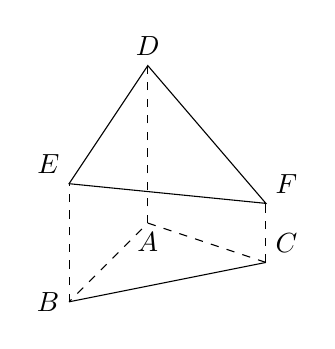
\begin{tikzpicture}[scale=0.5]
			\coordinate[label=left:$B$]  (B) at (0,0);
			\coordinate[label=above right:$C$]  (C) at (5,1);
			\coordinate[label=below:$A$]  (A) at (2,2);
			\coordinate[label=above:$D$]  (D) at (2,6);
			\coordinate[label=above left:$E$]  (E) at (0,3);
			\coordinate[label=above right:$F$]  (F) at (5,2.5);
			\draw (B) -- (C);
			\draw[dashed] (C)-- (A) -- (B);
			\draw[dashed] (A) -- (D);
			\draw[dashed] (B) -- (E);
			\draw[dashed] (C) -- (F);
			\draw (D) --(E)--(F)--cycle;
		\end{tikzpicture}
	\end{center}

		\begin{parts}
			\part Il vettore $\vec{v}=\vvec{-3,-15,12}$ è parallelo al lato $AB$?
			\rsol{Si}
			\part Il punto $K(1;9;-1)$ è allineato con $A$ e $B$?
			\rsol{No}
			\part Determinare la coordinata $z$ del punto $D$ in modo che il tronco di prisma sia retto.
			\rsol{$z=5$}
			\part

			Determinare le coordinate dei punti $E$ e $F$.
			\rsol{$E(5;1;-\frac{25}{2})$

				$F(4;4;0)$}

		\end{parts}


	\end{qblock}


	\begin{qblock}
		\question
		\exonly{
			Una padella di \SI{8}{\kilo\gram} è sospesa sopra il fuoco per mezzo di tre aste, fissate alla padella nei punti $A(0.00;0.44;0.40)$, $B(0.38;-0.22;0.40)$ e $C(-0.38;-0.22;0.40)$, i quali formano un tetraedro di vertice $V(0.00;0.00;1.022)$ tramite il quale la struttura è fissata al soffitto.

			Fare un schizzo della situazione e determinare le forze che sollecitano le aste.


		}

		\solonly{

			Versore: $\hat{AV}=\dfrac{\overrightarrow{AV}}{\norm{AV}}$
			Vincolo:


			$k_1 \cdot \hat{AV}+k_2 \cdot \hat{BV} +k_3 \cdot \hat{CV} + 8\cdot 9.81 \cdot \vvec{0,0,-1}=\vec{0}$

			$k_1=k_2=k_3\approx \qty{32}{\newton}$

		}
	\end{qblock}
\end{questions}

\subsection{Equazione vettoriale della retta}

\begin{questions}


	\begin{qblock}
		\question
		\exonly{Determinare un'equazione vettoriale della retta passante per i punti $A(-1;5)$ e $B(4;6)$}
		\solonly{$\vecII{x}{y}=\vecII{-1}{5}+\lambda \vecII{5}{1}$}
	\end{qblock}


	\begin{qblock}
		\question
		\exonly{Determinare un'equazione vettoriale della retta passante per $A(8;-1)$ e $B(2;7)$ e la sua distanza dal punto $C(7;17)$}

		\solonly{$\vvec{x,y}=\vvec{8,-1}+ \lambda \vvec{-6,8}$ \\ Distanza:$10$}
	\end{qblock}


	\begin{qblock}
		\question
		\exonly{Determinare la distanza della retta $4x+3y+9=0$ dal punto $C(3;-2)$}

		\solonly{$3$}
	\end{qblock}


	\begin{qblock}
		\question
		\exonly{Dato il quadrilatero $ABCD$ con $A(-2; -1)$, $B(6; 1)$, $C(5; 5)$ e $D(-1; 3)$}
		%\solonly{\hfill}

		\begin{parts}
			\part
			\exonly{Determinare il punto d’intersezione delle due diagonali}
			\solonly{$(\num{1.75};\num{2.21})$}

			\part
			\exonly{Determinare l’angolo acuto che formano le due diagonali tra di loro}
			\solonly{$\num{56.54}\degree$}

			\part
			\exonly{Determinare la distanza tra il punto d’intersezione e la retta passante per $A$ e $D$}
			\solonly{$\approx \num{2.9}$}

			\part

			\exonly{Determinare l’area del quadrilatero}
			\solonly{$\num{28}$}
		\end{parts}
	\end{qblock}


	\begin{qblock}
		\question
		\exonly{Determinare un'equazione vettoriale della retta passante per i punti $A(-1;5;4)$ e $B(4;6;-8)$}
		\solonly{$\vvec{x,y,z}=\vvec{-1,5,4}+\lambda \vvec{5,1,-12}$}
	\end{qblock}


	\begin{qblock}
		\question
		\exonly{Dato il quadrilatero $ABCD$ con $A(-2; -1;4)$, $B(6; 1;-2)$, $C(5; 5;1)$ e $D(\frac{3}{2};4;4)$}
		%\solonly{\hfill}

		\begin{parts}
			\part
			\exonly{Determinare il punto d’intersezione delle due diagonali. Se non hai trovato nessuna intersezione spiega il perché?}
			\solonly{$S=\emptyset$}

			\part Se non hai trovato nessuna intersezione prova con $D_1(1;4;4)$
			\solonly{$(\frac{8}{3};3;2)$}

			\part
			\exonly{Determinare l’angolo acuto che formano le due diagonali tra di loro}
			\solonly{$\num{64.44}\degree$}

			\part
			\exonly{Determinare la distanza tra il punto d’intersezione e la retta passante per $A$ e $D$}
			\solonly{$\approx \num{2.79}$}

			\part

			\exonly{Determinare l’area del quadrilatero}
			\solonly{$\num{36.59}$}
		\end{parts}
	\end{qblock}


	\begin{qblock}
		\question
		\exonly{Determinare la distanza della retta  $\vvec{x,y,z}=\vvec{1,2,5}+ \lambda \vvec{2,1,1}$ dal punto $P(-5;3;-1)$}
		\solonly{$\num{4.98}$}
	\end{qblock}


	\begin{qblock}
		\question
		\exonly{Determinare un'equazione vettoriale della retta passante per $A(8;-1;3)$ e $B(2;7;5)$ e la sua distanza dal punto $C(7;17;10)$}

		\solonly{$\vvec{x,y,z}=\vvec{8,-1,3}+ \lambda \vvec{-6,8,2}$ \\ Distanza: $10.74$}
	\end{qblock}

	\begin{qblock}
		\question
		\exonly{
			Determinare la distanza (minima) tra le due rette

			\nopagebreak
			$r_1:\vvec{x,y,z}=\vvec{1,2,3}+k_1\vvec{1,-1,2}$

			\nopagebreak
			$r_2:\vvec{x,y,z}=\vvec{1,3,1}+k_2\vvec{-1,3,-2}$

		}

		\nopagebreak
		\solonly{$\dfrac{2\sqrt{5}}{5}\approx 0.89$}

	\end{qblock}
\end{questions}
